% ==============================================================================
% Capítulo 4: Especificação de requisitos
% ==============================================================================
\chapter{Especificação de requisitos}
\label{cap:requisitos}

\begin{instrucao}
\orientacao{O que vai na Especificação de Requisitos}
Este capítulo descreve o que o sistema deve fazer e para quem. Inclua:
\begin{itemize}
  \item como os requisitos foram levantados (entrevistas, questionários,
        observação, análise de documentos) e com quem;
  \item os perfis de usuário e as partes interessadas;
  \item os requisitos funcionais, como casos de uso, histórias de usuário ou
        abordagem equivalente, conforme as competências do TCC;
  \item os requisitos não funcionais, escritos de forma verificável;
  \item as regras de negócio;
  \item os protótipos de interface usados para validar os requisitos.
\end{itemize}
Identifique cada requisito com um código (RF01, RNF01, RN01), porque eles
serão citados no projeto, na implementação e nos testes. Se a especificação
completa for longa, mantenha no texto os requisitos principais e coloque o
documento completo em um apêndice.
\end{instrucao}

Este capítulo apresenta os requisitos do Monitora. A
\cref{sec:requisitos:levantamento} descreve como eles foram levantados, as
\cref{sec:requisitos:funcionais,sec:requisitos:naofuncionais} apresentam os
requisitos funcionais e não funcionais e a \cref{sec:requisitos:prototipo}
mostra o protótipo de interface usado para validá-los.

% ------------------------------------------------------------------------------
\section{Levantamento e perfis de usuário}
\label{sec:requisitos:levantamento}

Os requisitos foram levantados em entrevistas semiestruturadas com quatro
monitores das disciplinas de Programação I e Estrutura de Dados I e com os dois
professores que os supervisionam. As entrevistas duraram cerca de 30 minutos
e seguiram um roteiro com perguntas sobre como os atendimentos são marcados,
registrados e relatados. Foram identificados três perfis de usuário:
\begin{alineas}
  \item \textbf{estudante}: consulta os horários disponíveis, reserva e cancela
        atendimentos;
  \item \textbf{monitor}: publica seus horários, confirma a presença dos
        estudantes e registra o assunto de cada atendimento;
  \item \textbf{professor}: cadastra os monitores da disciplina e consulta os
        relatórios de frequência e de assuntos atendidos.
\end{alineas}

% ------------------------------------------------------------------------------
\section{Requisitos funcionais}
\label{sec:requisitos:funcionais}

Os \acp{rf} foram registrados como histórias de usuário \cite{cohn2004user} e
priorizados com os professores supervisores em alta, média e baixa
prioridade. O \cref{qua:historias} apresenta as histórias de alta e média
prioridade, implementadas nesta versão do sistema.

\begin{quadro}[htbp]
  \centering
  \caption{Histórias de usuário do Monitora}
  \label{qua:historias}
  \small
  \begin{tabularx}{\textwidth}{|c|X|c|}
    \hline
    \textbf{Código} & \textbf{História de usuário} & \textbf{Prioridade} \\
    \hline
    RF01 & Como monitor, quero cadastrar meus horários semanais de atendimento
      para que os estudantes saibam quando estou disponível. & Alta \\
    \hline
    RF02 & Como estudante, quero ver os horários livres de uma disciplina para
      escolher o mais conveniente. & Alta \\
    \hline
    RF03 & Como estudante, quero reservar um horário para garantir meu
      atendimento. & Alta \\
    \hline
    RF04 & Como estudante, quero cancelar uma reserva para liberar o horário
      para outro colega. & Alta \\
    \hline
    RF05 & Como monitor, quero registrar a presença e o assunto de cada
      atendimento para compor meu relatório mensal. & Alta \\
    \hline
    RF06 & Como professor, quero cadastrar os monitores da minha disciplina para
      que eles possam publicar horários. & Média \\
    \hline
    RF07 & Como professor, quero emitir o relatório de frequência de cada
      monitor para comprovar as horas trabalhadas. & Média \\
    \hline
    RF08 & Como estudante, quero receber um lembrete na véspera do atendimento
      para não esquecer o compromisso. & Média \\
    \hline
  \end{tabularx}
  \fonteautor
\end{quadro}

Cada história tem critérios de aceitação que orientaram os testes. Para a
RF03, por exemplo, foram definidos os seguintes critérios:
\begin{alineas}
  \item a reserva só é aceita se o horário estiver livre;
  \item o estudante não pode ter duas reservas no mesmo horário;
  \item após a reserva, o horário deixa de aparecer como livre para os demais
        estudantes.
\end{alineas}

\begin{instrucao}
\orientacao{Histórias de usuário, casos de uso e critérios de aceitação}
Escolha uma forma de especificação e use-a de modo consistente. Histórias de
usuário são adequadas a processos ágeis. Casos de uso, com diagrama e
descrição textual (atores, pré-condições, fluxo principal e fluxos
alternativos), são adequados quando há muitos fluxos alternativos ou regras
complexas. Em ambos os casos, escreva critérios de aceitação verificáveis,
porque eles orientam os testes descritos no \cref{cap:testes}.
\end{instrucao}

% ------------------------------------------------------------------------------
\section{Requisitos não funcionais e regras de negócio}
\label{sec:requisitos:naofuncionais}

Os \acp{rnf} foram definidos de forma que pudessem ser verificados ao final do
desenvolvimento:
\begin{alineas}
  \item \textbf{RNF01 (usabilidade)}: o sistema deve obter pontuação média
        igual ou superior a 70 na escala \acs{sus} em avaliação com usuários;
  \item \textbf{RNF02 (compatibilidade)}: a interface deve funcionar em
        telas a partir de 360 \emph{pixels} de largura, nas versões atuais dos
        navegadores Chrome, Firefox e Safari;
  \item \textbf{RNF03 (desempenho)}: as páginas de consulta de horários devem
        ser carregadas em menos de dois segundos com 100 usuários simultâneos;
  \item \textbf{RNF04 (segurança)}: o acesso deve exigir autenticação e cada
        perfil deve ter acesso apenas às funcionalidades que lhe competem;
  \item \textbf{RNF05 (manutenibilidade)}: o código deve seguir o guia de
        estilo PEP~8 \cite{vanrossum2001pep8} e ter cobertura de testes
        automatizados de pelo menos 80\%.
\end{alineas}

As principais regras de negócio são as seguintes. Um estudante pode ter no
máximo duas reservas ativas por disciplina (RN01). Cancelamentos devem ocorrer
com pelo menos duas horas de antecedência (RN02). Um atendimento não
registrado pelo monitor em até 48 horas é marcado como pendente no relatório
do professor (RN03).

\begin{instrucao}
\orientacao{Requisitos não funcionais verificáveis}
``O sistema deve ser rápido'' ou ``o sistema deve ser fácil de usar'' não são
requisitos verificáveis. Associe cada requisito não funcional a uma medida e
a um valor esperado, como nos exemplos acima. Assim, no \cref{cap:testes}, é
possível mostrar se cada um foi atendido. A norma ISO/IEC 25010 oferece um
vocabulário de atributos de qualidade que ajuda a organizá-los.
\end{instrucao}

% ------------------------------------------------------------------------------
\section{Protótipo de interface}
\label{sec:requisitos:prototipo}

Antes da implementação, foram elaborados protótipos de baixa fidelidade das
telas principais, apresentados aos monitores e professores para validar os
requisitos. A \cref{fig:prototipo} mostra o protótipo da tela de reserva. A
validação levou a duas mudanças. A primeira foi exibir os horários em grade
semanal, e não em lista. A segunda foi mostrar o nome do monitor em cada
horário, porque os estudantes preferem ser atendidos por monitores
específicos.

\begin{figure}[htbp]
  \centering
  \caption{Protótipo de baixa fidelidade da tela de reserva de horários}
  \label{fig:prototipo}
  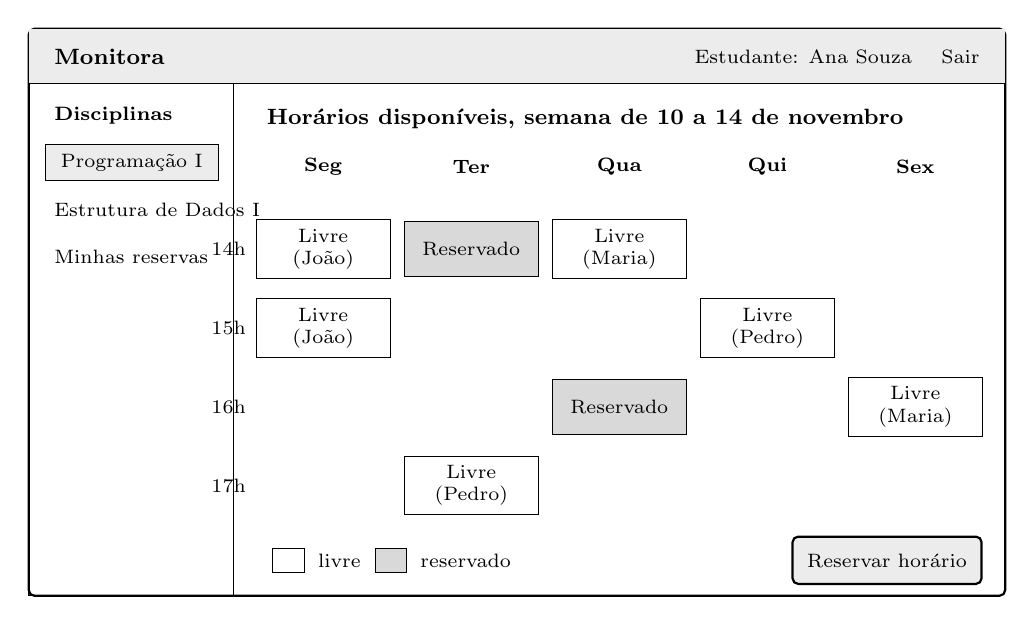
\begin{tikzpicture}[
      font=\scriptsize,
      livre/.style={draw, fill=white, minimum width=1.7cm, minimum height=7mm, align=center},
      ocupado/.style={draw, fill=gray!30, minimum width=1.7cm, minimum height=7mm, align=center},
    ]
    % janela
    \draw[thick, rounded corners=2pt] (0,0) rectangle (12.4,7.2);
    \fill[gray!15] (0,6.5) rectangle (12.4,7.2);
    \draw (0,6.5) -- (12.4,6.5);
    \node[anchor=west, font=\footnotesize\bfseries] at (0.2,6.85) {Monitora};
    \node[anchor=east] at (12.2,6.85) {Estudante: Ana Souza \quad Sair};
    % menu lateral
    \draw (0,0) rectangle (2.6,6.5);
    \node[anchor=west, font=\scriptsize\bfseries] at (0.2,6.1) {Disciplinas};
    \node[anchor=west, draw, fill=gray!15, minimum width=2.2cm] at (0.2,5.5) {Programação I};
    \node[anchor=west] at (0.2,4.9) {Estrutura de Dados I};
    \node[anchor=west] at (0.2,4.3) {Minhas reservas};
    % grade semanal
    \node[anchor=west, font=\footnotesize\bfseries] at (2.9,6.05) {Horários disponíveis, semana de 10 a 14 de novembro};
    \foreach \d [count=\i] in {Seg, Ter, Qua, Qui, Sex} {
      \node at (1.86+\i*1.88, 5.45) {\textbf{\d}};
    }
    \foreach \h [count=\j] in {14h, 15h, 16h, 17h} {
      \node[anchor=east] at (2.88, 5.4-\j*1.0) {\h};
    }
    \node[livre]   at (3.74,4.4) {Livre\\(João)};
    \node[ocupado] at (5.62,4.4) {Reservado};
    \node[livre]   at (7.50,4.4) {Livre\\(Maria)};
    \node[livre]   at (3.74,3.4) {Livre\\(João)};
    \node[livre]   at (9.38,3.4) {Livre\\(Pedro)};
    \node[ocupado] at (7.50,2.4) {Reservado};
    \node[livre]   at (11.26,2.4) {Livre\\(Maria)};
    \node[livre]   at (5.62,1.4) {Livre\\(Pedro)};
    % legenda e botão
    \node[draw, fill=white, minimum width=4mm, minimum height=3mm] at (3.3,0.45) {};
    \node[anchor=west] at (3.55,0.45) {livre};
    \node[draw, fill=gray!30, minimum width=4mm, minimum height=3mm] at (4.6,0.45) {};
    \node[anchor=west] at (4.85,0.45) {reservado};
    \node[draw, thick, rounded corners=2pt, fill=gray!15, minimum width=2.4cm, minimum height=6mm] at (10.9,0.45) {Reservar horário};
  \end{tikzpicture}
  \fonteautor
\end{figure}

\begin{instrucao}
\orientacao{Protótipos}
Protótipos ajudam a validar requisitos antes de implementar e mitigam o risco
de construir algo que os usuários não querem, como pedem as competências do
TCC. Podem ser esboços em papel fotografados, telas feitas no Figma ou no
Penpot (exportadas em PDF ou SVG) ou desenhos simples em TikZ, como a
\cref{fig:prototipo}. Relate o que mudou nos requisitos a partir da validação
com os usuários.
\end{instrucao}
